Modelis yra būtinas, norint atlikti filtravimo operaciją.
Modelis apibūdina nagrinėjamą sistemą, kokios komponentės, kaip priklauso nuo esamų parametrų.

\subsection{Pradinis modelis}

Jutiklio duomenys gražina pagreičio vertes, o užduotis yra nustatyti poziciją. 
Pozicijos pokytis priklauso $s(t)$ nuo objekto greičio $v(t)$.

\begin{equation}
    s(t) = \int_0^tv(t) \delta t
\end{equation}

Tuo tarpu greitis duotu laiko momentu $v(t)$ priklauso nuo pagreičio $a(t)$.

\begin{equation}
    v(t) = \int_0^t a(t) \delta t
\end{equation}

Iš to seka, kad norint gauti sistemos poziciją, pagreitį reikia integruoti du kartus

\begin{equation}
    s(t) = \int_0^tv(t) \delta t = \int_0^t \int_0^t a(t) \delta t \delta t
\end{equation}

Tokiu būdu gaunamas paprasčiausias matematinis modelis, kurio naudojantis galima nustatyti dabartinę objekto poziciją.
Didžiausias šito modelio trūkumas yra dvigubas integravimas.
Pagreitis turi labai didelį matavimo triukšmą.
Integruojant vieną kartą, triukšmo įtaka matavimui yra padidinama du kartus.
Integruojant du kartus -- triukšmas padidėja keturis kartus. 
Šis modelis bus naudojamas tolimesniame darbe kaip palyginimas su filtrais.

\subsection{Kalman filtro modelis}

Kalman filtras reikalauja modelį aprašyti lygčių sistemą.
Jinai turi apibūdinti atliekamus matavimus, bei norimą pasiekti rezultatą, kuris priklauso nuo atliekamų matavimų.
Pagreičio lygtis yra labai paprasta, kadangi pagreitis yra tiesioginis sistemos matavimas

\begin{equation}
    a(t) = a(t)
\end{equation}

Greitis priklauso nuo greičio, kuris buvo vienu laiko momentu prieš, ir nauju pagreičiu

\begin{equation}
    v(t) = v(t-1) + a(t) * \delta t
\end{equation}

Pozicija priklauso nuo prieš tai buvusios pozicijos, dabartinio greičio poslinkio, bei pagreičio kvadrato

\begin{equation}
    s(t) = s(t-1) + v(t-1) + \frac{a(t)}{2}\delta t^2
\end{equation}

Iš šitų lygčių yra sudaromas sistemos būsenos modelis

\begin{equation}
    \hat{x} = \begin{cases}
        s(t-1) + v(t-1) + \frac{a(t)}{2}\delta t^2 \\
        v(t-1) + a(t) * \delta t \\
        a(t)
    \end{cases}
\end{equation}

Kadangi iš viso mes turime tris ašis, modelis patrigubėja ir iš viso jį sudaro

\begin{equation}
    \hat{x} = [ x, y, z, \dot{x}, \dot{y}, \dot{z}, \ddot{x}, \ddot{y}, \ddot{z}]^T,
\end{equation}
kur $\dot{x}$ yra pozicijos pirmą išvestinė -- greitis, $\ddot{x}$ yra pozicijos antra išvestinė -- pagreitis.

Galutinė sistemos būsenos matrica atrodo

\begin{equation}
    F = \begin{bmatrix}
        1 & 0 & 0 & dT & 0 & 0 & \frac{\delta dT^2}{2} & 0 & 0 \\
        0 & 1 & 0 & 0 & dT & 0 & 0 & \frac{\delta dT^2}{2} & 0 \\
        0 & 0 & 1 & 0 & 0 & dT & 0 & 0 & \frac{\delta dT^2}{2} \\
        0 & 0 & 0 & 1 & 0 & 0 & dT & 0 & 0 \\
        0 & 0 & 0 & 0 & 1 & 0 & 0 & dT & 0 \\
        0 & 0 & 0 & 0 & 0 & 1 & 0 & 0 & dT \\
        0 & 0 & 0 & 0 & 0 & 0 & 1 & 0 & 0 \\
        0 & 0 & 0 & 0 & 0 & 0 & 0 & 1 & 0 \\
        0 & 0 & 0 & 0 & 0 & 0 & 0 & 0 & 1
    \end{bmatrix},
\end{equation}
kur $dT$ yra laiko pokytis tarp matavimų.

Kalman filtro veikimui yra reikalauja turėti matavimų matricą.
Matavimų matrica nurodo, kuris iš modelio komponentų yra pats matavimas.
Šiuo atveju egzistuoja trys pagreičio komponentės, kurios nusako atliekamus matavimus.

\begin{equation}
    H = \begin{bmatrix}
        0 & 0 & 0 & 0 & 0 & 0 & 1 & 0 & 0 \\
        0 & 0 & 0 & 0 & 0 & 0 & 0 & 1 & 0 \\
        0 & 0 & 0 & 0 & 0 & 0 & 0 & 0 & 1
    \end{bmatrix}
\end{equation}

Tokios modelio informacijos pakanka Kalman filtro darbui. 
Grafike \ref{fig:two_dimensional_kalman_filter} yra parodytas Kalman atlikto signalo filtravimo pavyzdys.

\begin{figure}[H]
    \centering
    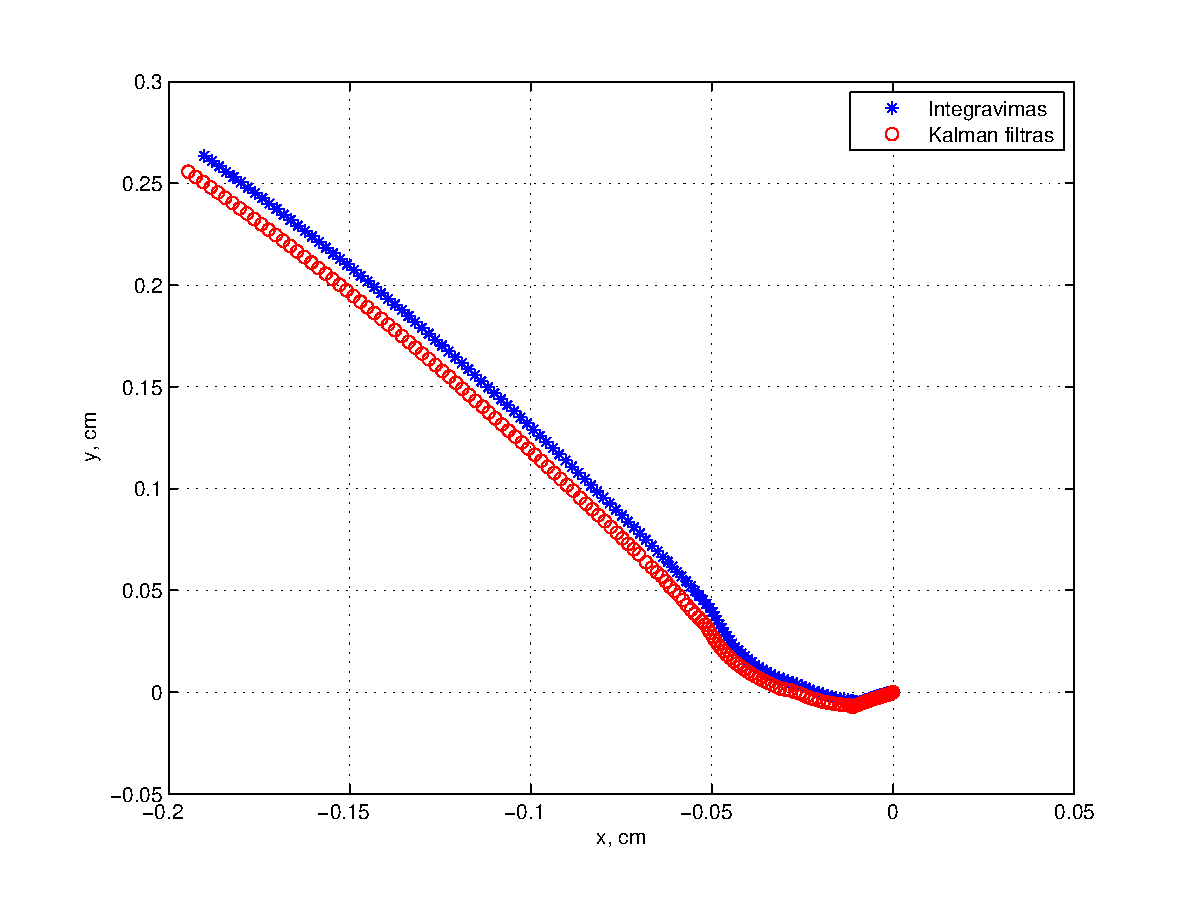
\includegraphics[
        width=0.8\textwidth
    ]{img/kalman_1.eps}
    \caption{Kalman filtro signalo filtravimas dviejų dimensijų plokštumoje}
    \label{fig:two_dimensional_kalman_filter}
\end{figure}

